\chapter{Algorithms}
\label{chapter:algorithm}

Section~\ref{sec:theoritical_background} in contraction describes different methods that we propose to use in this work. After the brief discussion about the data and theory in previous sections we will now, in this section develop the analysis pipelines for both our proposed methods and elaborate on the components of involved analysis system. The clarity of data flow in the pipelines ensured by talking about the components as algorithmic modules.


\section{Patch Based Dictionary Learning Pipeline}
\label{sec:scc}

This section introduces the computational algorithms of the patch based dictionary learning and sparse coding procedures in detail . Major steps are summarized in Alg. \ref{alg:pipeline1} and Fig. \ref{fig:pipeline1}. 

\subsection{Patch Generation for Dictionary Learning}
\label{subsec:Patch_Generation_Dictionary_Learning}
In the first pipeline to find a better representation of the data in low class-separability groups we will use Stochastic Coordinate Coding (SCC) to learn the sparse representation of the FDG-PET scans. We generate 8000 image patches of dimension $ 10 \times 10 \times 10 $ in each FDG-PET image, $ x_i \in R^{1 \times p} $ where $ i \in \{ 1 \dots n \}$. Of these we select $2000$ patches to initialize the dictionary. This arrangement would ensure overlapping which is proven to be very efficient in practice~\citep{lin2014stochastic,zhang2016applying}. We generalize a cost function $ X = (x_1,x_2,\dots,x_n) $, where $ n $ is the number of patches and $ p $ is the patch dimension. As we noted early during experimentation the patch dimension is $1000$ and the objective matrix for SCC is thus $samples*no~of~patches \times patch~dimension $. The number of elements in an experiment is close to half a billion (644,000,000 in case of AD vs. Normal) given the limit of space and complexity we decide to downsample the patch dimension using max-pooling with a $ 2 \times 2 \times 2 $ window. The new size of patch is now $ 125 $. 

\begin{algorithm}
	\vspace{1em}
	\caption{Patch Based Stochastic Coordinate Coding}\label{alg:pipeline1}
	
	\KwIn{A number of FDG-PET images}
	
	\KwOut{A set of features and labels for the six classification experiment}
	
	The segmented dataset is divided and segregated into 6 binary parcels
	
	\For{exp $ \gets $ \{ [AD vs. CU], [AD vs. EMCI], [AD vs. LMCI], [CU vs. EMCI], [CU vs. LMCI], [EMCI vs. LMCI]. \}} {
		
		m $ \gets $ number of samples
		
		n $ \gets $ number of patches
		
		p $ \gets $ patch dimension
		
		Initialize X = [m*n $ \times $ p]
		\For{samples $ \in $ exp}{
			A three dimensional patch of 10 $ \times $ 10 $ \times $ 10 is created in order to extract meaning full information from the 3D segmented PET scans.   
		
	    	A number of random patches are generated over the volume and random meaningful patches are selected from the ROI to initialize the dictionary. 
	
			\For{patch $ \in $ patches}{
				 downsample ``patch'' \& linearly rearranged $ X_{patch} = (x_1,\dots,x_p)$ where $ patch \in p$.
			
				A matrix of all patches is arranged. i.e., X[sample*patch, : ] = [ $X_{patch}$']
			}
	}

	$ X $ is then fed into the stochastic coordinate coding module. (Fig. \ref{fig:pipeline1}(c)).
	
	We apply max-pooling algorithm on the learned 2000-dimension dictionary to aggregate discriminant features (Fig. \ref{fig:pipeline1}(d)).
	
	Ada-Boost is used to classify the six binary classification experiments. 
	}
\end{algorithm}


\subsection{Finding Dictionary and Sparse Codes}
\label{sec:dictionary_learning}
Dictionary learning is the learning of the basis set, also called the dictionary, to adapt it to specific data, an approach that has recently proven to be very effective for signal processing in the audio and image processing domains. Different from traditional feature extraction methods like principle component analysis and its variants, sparse coding learns non-orthogonal and over-complete dictionaries which have more flexibility to represent data. Stochastic Coordinate Coding  has been used successfully in the past~\citep{lin2014stochastic,mairal2009online}.

The following section describes Stochastic Coordinate Coding (SCC) algorithm~\citep{lin2014stochastic}. The dictionary is initialized via any initialization method and denoted as $ D_1^1 $. The sparse codes are initialized as $ z_i^0 = 0 $ for $ i=1,\dots,n $. Where $ i $ is the index of data points and the superscript denotes the number of epoch. The algorithm is describes as follows:\\
(1). Get an image patch $ x_i $.\\
(2). Update $ z_i^k $ via one or a few steps of coordinate descent: 
\begin{equation}
z^k_i = CD(D^k_i,z^{k-1}_i,x_i).
\end{equation}
Specifically, for $ j $ from 1 to $ m $, update the $ j $-th coordinate $ z_{i,j}^{k-1} $ of $ z_{i}^{k-1} $ cyclically as follows:
\begin{equation}
b_j \gets (d_{i,j}^k)^T (x_i - D_i^kz^{k-1}_i) + z^{k-1}_{i,j}, z_{i,j}^{k-1} \gets h_{\lambda}(b_j),
\end{equation}	
where h is the soft thresholding shrinkage function. We call such cycle as one step of coordinate descent. The updated sparse code is then denoted by $ z_i^k $. \\
(3). Update the dictionary $ D $ by using stochastic gradient descent:
\begin{equation}
D_{i+1}^k = P_{B_m}(D_i^k - \eta^k_i\Delta_{D_i^k} f_i(D_i^k,z^k_i))
\end{equation}

where $ P $ denotes the projection operator. We set the learning rate as an approximate of the inverse of the Hessian matrix. The gradient of $ D_i^k $ can be obtained as follows:

\begin{equation}
\Delta_{D_i^k} f_i (D_i^k, z_i^k) = (D^k_iz^k_i - x_i)(z^k_i)^T.
\end{equation}

(4). $ i = i+1 $. If $ i \ge n $, then set $ D_1^{k+1} = D^k_{n+1}, ~k=k+1$ and $ i = 1 $.

When the data sets are very large, the learning rate $ \eta^k_i $ will be very small. In this case, the dictionary will not change very much and the efficiency of the training will decrease. In practice tuning the learning rate is tricky and sensitive. To obtain the learning rate we use the Hessian matrix of the objective function. It is shown that the following matrix provides an approximation of the Hessian: $ \mathbf{H} = \sum_{k,i} z^k_i(z^k_i)^T $, when $ k $ and $ i $ go to infinity. According to the second order stochastic gradient descent, we should use the inverse matrix of the Hessian as the learning rate. However, computing a matrix inversion problem is computationally expensive. In order to get the learning rate, we simply use the diagonal elements of the matrix $ H $. The matrix $ H $ is updated as follows:
\begin{equation}
H \gets H + z^k_i(z^k_i)^T.
\end{equation}

Alg. \ref{alg:scc} summarizes the steps described in section \ref{sec:dictionary_learning}

\begin{algorithm}
	
	\caption{SCC (Stochastic Coordinate Coding)}\label{alg:scc}
	
	\KwIn{Data set $ X = (x_1,x_2,\dots,x_n) \in R^{p \times n} $, ensure $ D \in R^{p \times m} $ and $ Z =  (z_1 \dots z_n ) \in R ^{m \times n}$}
	\KwOut{$ D = D^k_n$ and $z_i = z_i^k $ for $ i = i,\dots,n $.}
	
	Initialize $ D_1^1, H = 0 $ and $ z_i^0 $ for $ i = 1,\dots,n $,
	
	\For{$ k = 1 $ to $ k $ do }
	{\For{$ i = 1$ to $ n $}
		{Get an image patch $ x_i $\\
			Update $ z_i^k $ via one or a few steps of coordinate descent: \hspace{1.5cm}$ z_i^k \gets CD(D_i^k,z^{k-1}_i,x_i)$.\\
			Update the Hessian matrix and the learninig rate:
			\hspace{1.5cm}$ H \gets H + z^k_i(z^k_i)^T, ~\eta^k_{i,j} = \frac{1}{h_{jj}} $.\\
			Update the support of the dictionary via SGD:
			\hspace{1.5cm}$ d^k_{i+1,j} \gets d^k_{i,j} - \eta^k_{i,j}z_{i,j}(D_i^kz^k_i - x_i) $\\
			If $ i = n $, set $ D_1^{k+1} = D^k_{n+1} $.
		}
	}
	
\end{algorithm}

\pagebreak
\section{Patch Based Dimensionality Reduction Pipeline}
\label{sec:dimension_reduction}

This section introduces the computational algorithms of the patch based feature extraction (dimensionality reduction) classification procedures in detail. Major steps are summarized in Alg.~\ref{alg:pipeline1} and Fig. \ref{fig:pipeline2}. 

\subsection{Patch Generation and Feature Selection}
\label{subsec:patch_generation}
After we identify the region of interest as the cerebral cortex in the FDG-PET scans we are left with a 80 $ \times $ 95 $ \times $ 80 voxel intensities which represent the metabolic activity. For this study we choose the entire cerebral cortex as the basis for comparison or as we would call it the biomarker. The feature dimension with the FDG-PET data is much larger than the number of subjects and is therefore prone to overfitting. We first randomly generate a number of small 10 $ \times $ 10 $ \times $ 10 windows on each image volume to obtain a collection of small image patches with different amounts of overlap. The procedure is in fact equivalent to applying a high-pass filter to the original volume. As a result, the region of interest (ROI) are still present, but some low frequency signals have disappeared. 

In the first pipeline we pool and arranged the patches into a linear array $ X_i = (x^1_i,\dots,x^n_i) $ where $ n $ is the number of feature and $ i \in \{1 \dots m\} $, where $ m $ is the number of samples in a group and stack them for the concerned group $ X = (X_1,\dots,X_i,\dots,X_m) $. The corresponding labels are also generated in this step $ Y = (y_1,\dots,y_m) $. We will then try to find out the linear and non-linear separability of the data using machine learning algorithms.

Illustration of the patch selection procedure is shown in Fig. \ref{fig:patches} (b).

\begin{algorithm}
	\vspace{1em}
	\caption{Patch Based Feature Extraction \& Dimensionality Reduction Pipeline}\label{alg:pipeline2}
	
	\KwIn{A number of FDG-PET images}
	
	\KwOut{A set of features and labels for the six classification experiment}
	
	The segmented dataset is divided and segregated into 6 binary parcels.
	
	\For{exp $ \gets $ \{ [AD vs. CU], [AD vs. EMCI], [AD vs. LMCI], [CU vs. EMCI], [CU vs. LMCI], [EMCI vs. LMCI]. \}} {
		
		n $ \gets $ number of samples
		
		p $ \gets $ number of patches
		
		Initialize X = [n $ \times $ p]
		
		\For{sample $ \in $ exp}{
			A three dimensional patch of 10 $ \times $ 10 $ \times $ 10 is created in order to extract meaning full information from the 3D segmented PET scan.   
			
			A number of patches are generated over the PET volume and overlapping is ensured
			
			All patch windows are max-pooled and linearly arranged into a vector $ B $(Fig.\ref{fig:pipeline2} (b)).  
			
			$ X_{sample} \gets $ B. Where sample $ \in $ m
		}
		
		In $ X $ the high dimensionality of the data is reduced by probabilistic PCA to avoid over fitting (Fig. \ref{fig:pipeline2}(c)).
		
		classification of $ X $: sample $ \times $ features, $ Y $: labels, is performed by AdaBoost. 
	}
\end{algorithm}


\subsection{Finding Linear Class Separability}
\label{sec:dicsriminant_analysis}

Having designed the training dataset $ X $ in section~\ref{subsec:patch_generation}, we can now use it for classification. However when a vast number of variables are measured from a relatively small dataset, the feature dimension is usually much larger than the sample size and the volume of the space increases so fast that the available data becomes sparse. In such a problem an enormous amount of data is required to ensure that there are several samples with each combination of values thus ensure no overfitting. With a fixed number of training samples, the predictive power reduces as the dimensionality increases. To overcome this issue we choose to effectively represent our data by reducing the dimensions of our feature space. In machine learning, dimensionality reduction is the introduction of new feature space where the original features are represented. The new space is of lower dimension that the original space. e.g., principle component analysis (PCA)~\citep{jolliffe2002principal}, linear discriminant analysis (LDA)~\citep{mika1999fisher}.

 A major limitation of traditional PCA is that it is non-parametric as there is no probabilistic model for observed data. In 1999 ME Tipping~\citep*{tipping1999mixtures} proposed a probabilistic PCA model (PPCA) in which the principle axes of a set of observed data vectors may be determined through maximum-likelihood estimation. The main idea of PPCA is based on the latent variable models which seeks to relate a $ d $-dimensional observed data vector $ \mathbf{t} $ to a corresponding $ q $-dimensional vector of latent variable (i.e. the unobserved variables that can be inferred from the model) $ x $.
\begin{equation}
\mathbf{y} = Wx + \mu + \epsilon
\end{equation} 
where, latent variables $ x \sim \mathcal{N}(0,I)) $. the noise model is described as $ \epsilon \sim \mathcal{N}(0,\Psi) $, and the ($ d \times q $) parameters matrix $ W $ contains the factor loading (Factor Analysis). $ \mu $ is the mean, given this formulation the observational vectors $ \mathbf{t} $ are also normally distributed $ \mathbf{t} \sim \mathcal{N}(\mu,C) $. In regards to equation (4.1) the probability model for the case of isotropic noise $ \epsilon \sim \mathcal{N}(0,\sigma^2I) $ is 
\begin{itemize}
	\item $ y|x \sim \mathcal{N}(WX + \mu, \sigma^2I) $
	\item $ y \sim \mathcal{N}(\mu, C_y) $, where $ c_y = WW^T + \sigma^2I $ (where $C_y$ is the covariance matrix for the observed data $ y $)
\end{itemize}
The Maximum Likelihood solution for PPCA is obtained as: \\$W_{MLE} = U_q(\Lambda_q - \sigma_{MLE}^2I)^{1/2}R$, \\where $U_q$ is a matrix of $q$ leading principal directions(eigen values of the covariance matrix), $\Lambda_q$ is a diagonal matrix of corresponding eigenvalues. \\$\sigma_{MLE}^2 = \frac{1}{d-q}\sum_{j=q-1}^{d}\lambda_j$ represents the variance lost in the projection and $R$ is an arbitrary $q\times q$ rotation matrix (corresponding to rotations in the latent space). 

A key motivation for this model is that because of the diagonality of $ \Psi $ (the variance not accounted by the latent factors ergo noise.) observed variables are conditionally independent given latent factors $ x $. The intention is that the dependencies between the data variables $t$ are explained by a smaller number of latent variables $x$, while $ \epsilon $ 
represents variance unique to
each observation variable, unlike PCA which treats covariance and variance similarly. 


\begin{figure}[h]
	\centering
	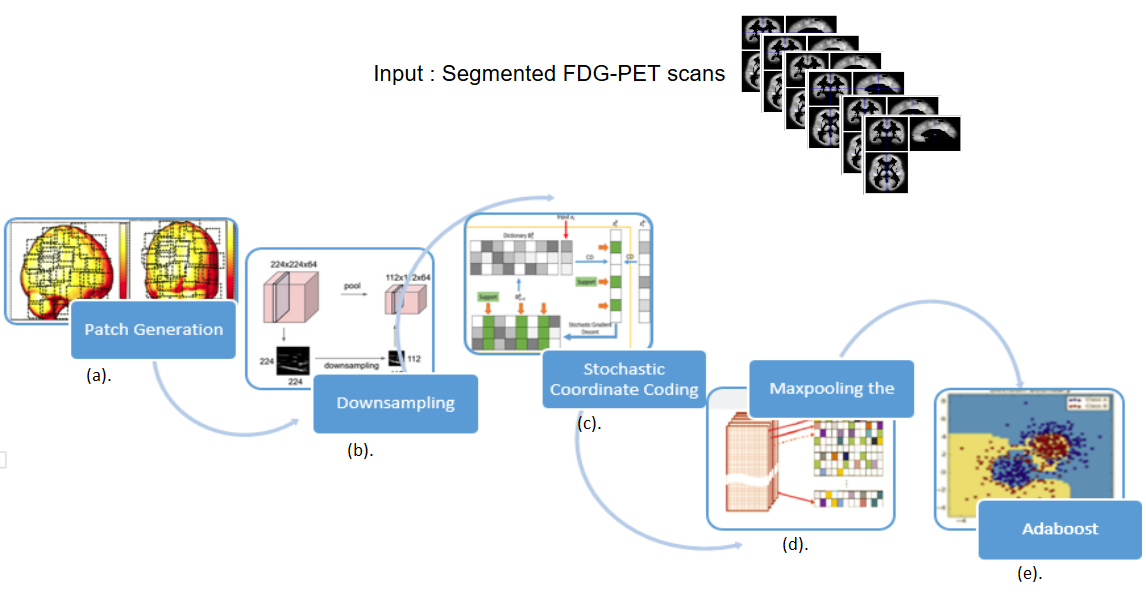
\includegraphics[width=\linewidth]{figures/pipeline1.png}
	\caption[Pipelines for Patch based Stochastic Coordinate Coding]{Pipelines for patch based Stochastic Coordinate Coding. (a). Patches are generated for feature extraction. (b). The size of patch dimension is reduced (c). After linearly arranging all the patches we find the dictionary and the sparse codes. (d). Maxpooling the learned sparse codes for obtaining a objective matrix. (e).applying AdaBoost for classification.}
	\label{fig:pipeline1}
\end{figure}

\begin{figure}[h]
	\centering
	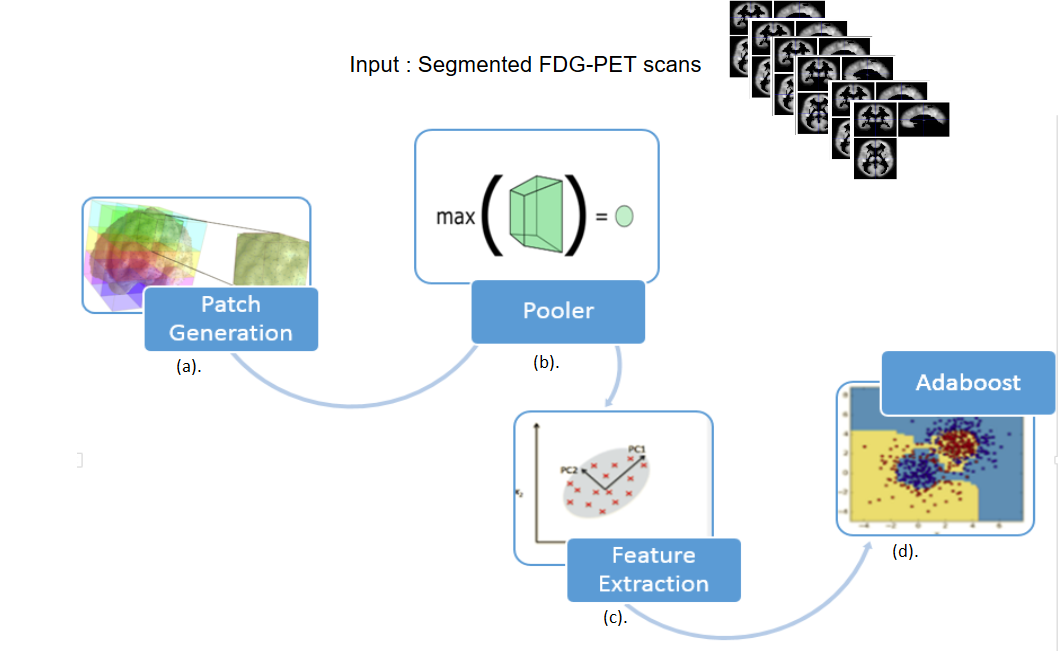
\includegraphics[width=\linewidth]{figures/pipeline2.png}
	\caption[Pipelines for Patch based Feature Extraction]{Pipelines for patch based feature extraction, (a). patches are generated for feature extraction. (b). patches are pooled to obtain specific activation. (c). the pooled values are linearly arranged and PCA is used to reduce it to a lower dimension space. (d). Adaboost is applied on the new feature space.}
	\label{fig:pipeline2}
\end{figure}

\section{Assumptions}
In both our methods we have made certain assumptions while building the system. This section describes the assumptions and to what extent they hold true 
\begin{enumerate}
\item \textit{The sample of the population is a representative sample.}\\
We assume the sample provided by the ADNI initiative is representative of the the population. The representative sample allows the collected results to be generalized to a larger population. We assume the \FDGPET~ analysis can be generalized to the general population.
\item \textit{3D Patch pooling represents the activation of a volume.}\\
In our first method of classification we use patch statistics to build the feature matrix with an assumption that the aggregate volume's (under $ 10\times10\times10 $) activation can be represented by the maximum intensity of the voxel within that region.   
\item \textit{The cerebral cortex intensities are assumed to serve as a biomarker.}\\
In this study we assume that the entire cerebral cortex may relay the metabolic information. In previous years z-score based t-values have been calculated to study regions of the brain and theory states that the metabolic changes during disease progression have a differential effect on various parts of the brain~\citep{ishii2014pet}. This is a benign analysis and we assume cerebral cortex is can serve as a good biomarker. 
\end{enumerate}
